%!TEX root = main.tex

\section{Variations}
\subsection{Weak o-minimality}

\begin{frame}[c]\frametitle{Weakly o-minimal structures}
	
	Let $\mathcal{M} = (M,<, \dots )$ be a linearly ordered structure.
    
	\begin{beamerboxesrounded}[shadow=true]{Definition}
		A set $C \subseteq M$ is called \em convex \em, if for any $a,b \in C$ with $a<b$, and $c\in M$ such that $a<c<b$, then $c \in C$. 
	\end{beamerboxesrounded}

	\begin{beamerboxesrounded}[shadow=true]{Definition}
		A structure $\mathcal{M}$ will be called \em weakly o-minimal \em, if the definable subsets of $\mathcal{M}$ are finite unions of convex sets in $(M,<)$.\\
		We say that a complete theory $T$ is \em weakly o-minimal \em if every model of $T$ is weakly o-minimal. 
	\end{beamerboxesrounded}

	\begin{beamerboxesrounded}[shadow=true]{Theorem}
		Expanding an o-minimal structure with unary predicates for convex subsets yields a structure with weakly o-minimal theory.
	\end{beamerboxesrounded}

\end{frame}

\begin{frame}[t]\frametitle{Monotonicity}
    \only<1>{
		Let $\mathcal{M}=(M,<,P,Q,f)$ such that.
		\begin{itemize}
			\item $M$ is the disjoint union of the interpretations of the unary relations $P$ and $Q$
			\item $P$ is the interpretation of $\mathbb{Q}$ with the usual order
			\item $Q$ is the interpretation of $\mathbb{Q} \times \mathbb{Q}$, lexicographically ordered
			\item $P$ proeceds $Q$ in $<$ on $M$ 
			\item $f:Q \to P$, $f((n,m))=n$ for all $n,m \in \mathbb{Q}$
		\end{itemize}
		$M$ is weakly o-minimal and also $\text{Th}(\mathcal{M})$ is weakly o-minimal.\\~\\
		}
	\only<2>{
		\begin{center}
			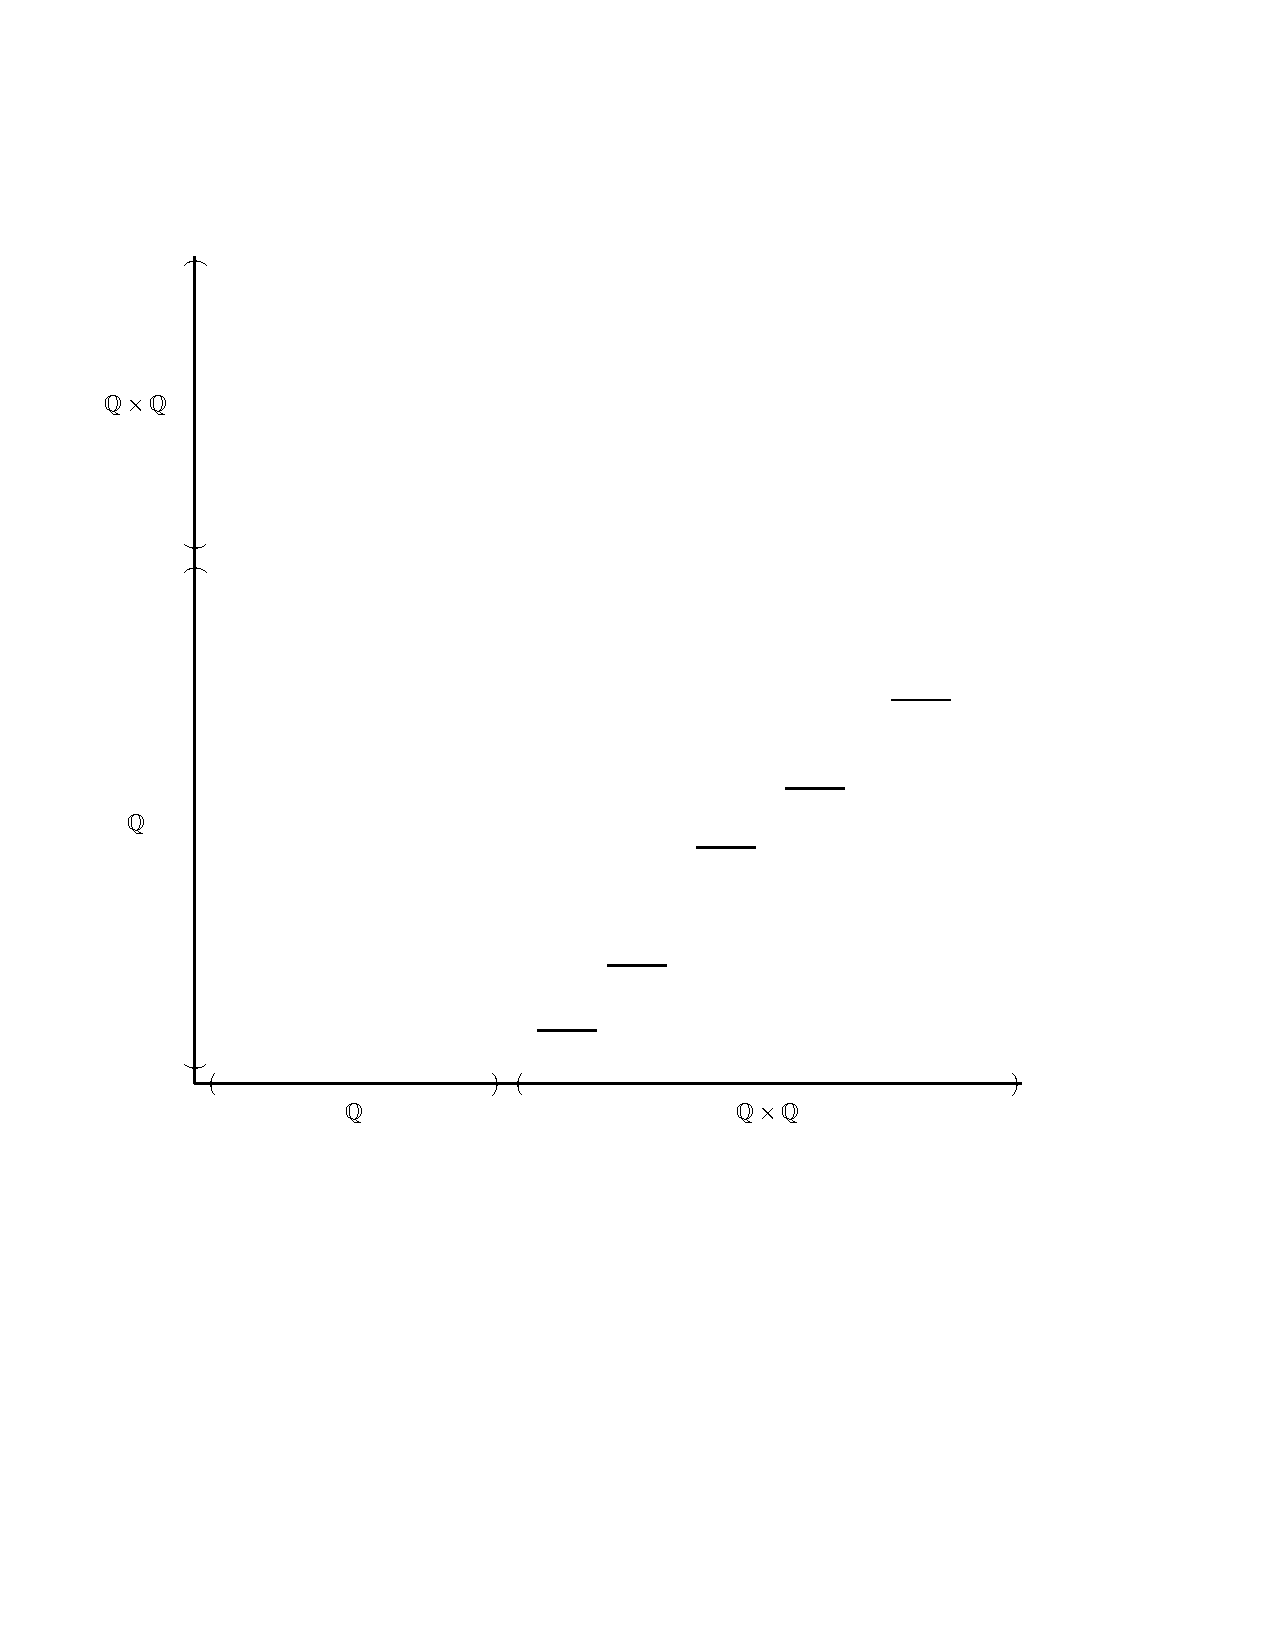
\includegraphics[height=7cm,width=7cm]{img/weakly-monotonicity--.pdf}
		\end{center}
	}

\end{frame}

\begin{frame}[t]\frametitle{Weakly o-minimal structures}

    
	\begin{itemize}
		\item[$\color{darkred}\bigstar$] We have a local monotonicity theorem.
		\item[$\color{darkred}\bigstar$] Weakly o-minimal structures do not neccesserily have weakly o-minimal theory.
		\item[$\color{darkred}\bigstar$] Weakly o-minimal structures do not neccesserily have prime models.
	\end{itemize}

	\begin{beamerboxesrounded}[shadow=true]{Theorem}
		Every weakly o-minimal ordered group is divisible and abelian.
	\end{beamerboxesrounded}

	\begin{beamerboxesrounded}[shadow=true]{Theorem}
		Every weakly o-minimal ordered field is real closed.
	\end{beamerboxesrounded}
\end{frame}

\subsection{Other variations}

\begin{frame}[t]\frametitle{A definition for minimality}
    
	Let $L\subset L^{+}$ be languages, and $\mathcal{K}$ be an elementary 
	class of $L$-structures.\\~\\
	\begin{beamerboxesrounded}[shadow=true]{Definition}
		An $L^{+}$-structure $\mathcal{M}$ is \em $\mathcal{K}$-minimal \em if the 
		the reduct $\mathcal{M}|_{L}$ is in $\mathcal{K}$ and every $L^{+}$-definable subset of $M$ is definable by a quantifier-free $L$-formula.\\
		A complete $L^{+}$-theory is \em $\mathcal{K}$-minimal \em if all its models are $\mathcal{K}$-minimal.
	\end{beamerboxesrounded}

	\begin{itemize}
		\item[$\color{darkred}\bigstar$] o-minimality is a special case of the above definition but not weak o-minimality.
		\item[$\color{darkred}\bigstar$] $\mathcal{K}$-minimality is closed under reducts to languages containg $L$, and under expansion by constants.
	\end{itemize}

\end{frame}

\begin{frame}[t]\frametitle{C-minimality}
    
	Let $C(x;y,z)$ be a ternary realation, $L=\{ C \}$, and $\mathcal{K}_{C}$ 
	be the class of $L$-structures satisfying the following axioms.

	\begin{itemize}
		\item $(\forall xyz)[C(x;y,z)\to C(x;z,y)]$
		\item $(\forall xyz)[C(x;y,z)\to C(y;x,z)]$
		\item $(\forall xyzw)[C(x;y,z)\to (C(w;y,z) \vee C(x;w,z))]$
		\item $(\forall xy)[x\neq y \to (\exists z \neq y)C(x;y,z)]$
		\item $(\exists xy)(x\neq y)$
	\end{itemize}

	\begin{beamerboxesrounded}[shadow=true]{Definition}
		A structure $\mathcal{M}=(M,C,\ldots)$ is \em $C$-minimal \em if 
		its theory is $\mathcal{K}_{C}$-minimal.
	\end{beamerboxesrounded}

\end{frame}

\begin{frame}[t]\frametitle{P-minimality}
    
	\begin{beamerboxesrounded}[shadow=true]{Definition}
		Let $L=(+,-,\cdot,0,1,(P_{n})_{n>1})$, where $P_n$ are unary
		predicates. Regard $\mathbb{Q}_p$ as an $L$-structure, letting $P_n$ picking the $n^{\text{th}}$ powers in $mathbold{Q_p}$.
		Let $\mathcal{K}_P$ be the class of $L$-structures elementarily equivalent to $\mathbb{Q}_p$. 
		Then if $L^{+}\supseteq L$, an $L^{+}$-structure is \em $P$-minimal \em
		if all models of its theory are $\mathcal{K}_P$-minimal
	\end{beamerboxesrounded}

\end{frame}